\chapter{Einleitung}
\label{cha:einleitung}

%    Umfeld definieren -> Warum SAP? Warum Bausparkasse? In das Thema hineinführen

    \section{Motivation und Ziel}
    \label{sec:motivation}

        Die SAP SE ist ein globaler Anbieter für Standardsoftware zur Unternehmenssteuerung und -kontrolle. In Kooperation mit einer Bausparkasse soll ein Modul entwickelt werden, dass die Abwicklung von Bauspar- und Baufinanzierungsverträgen vereinfacht. Dabei werden von Seiten der Bausparkasse hohe Anforderungen hinsichtlich der Qualität der Lösung gestellt, da Softwarefehler in einem Finanzinstitut sehr teuer sein können.

        \begin{quote}
          \enquote{32\% aller Projekte werden im Zeitplan, im Budget und entsprechend der Erwartungen fertig gestellt.}\footnote{Standish Group (CHAOS Summary), S.1.}
        \end{quote}

        Um den Anteil der 68\% an zu teuren, zu langsamen oder unfertigen Softwareprojekten nicht zu vergrößern, sollen agile Entwicklungsverfahren verwendet werden, die eine bessere Planbarkeit versprechen und unabhängig von der Projektdauer ein getestetes und lauffähiges Produkt bereitstellen. Die Prüfung der Software, die sich bei traditionellen Softwareentwicklungsmodellen an die Entwicklung anschließt, ist sehr schwer zu planen, da die Zahl der zu korrigierenden Fehler im Vorhinein nicht festzulegen ist.

        Als Antwort auf diese Problematik wurden agile Projektmethoden entwickelt, die die Projekte deutlich flexibler und planbarer machen sollen. Daher wurde entschieden, dass das betrachtete Projekt agil gestaltet wird.
        Bei agilen Methoden wird die Software in Bausteine aufgebrochen, die in kurzen Iterationen entworfen, implementiert und getestet werden. Am Ende jeder Iteration steht ein fertiger Baustein der finalen Software, der mit den restlichen Bausteinen das Endprodukt bildet. Da jeder Baustein in sich geschlossen eine Funktionalität anbietet, gibt es zum Schluss einer Iteration meist ein lauffähiges Produkt.

        Doch wie lässt sich sicherstellen, dass die Bausteine zu einander passen? Wie wird der Fortschritt des Projektes während der Laufzeit geprüft? Wie kann der Projektplan frühzeitig angepasst oder das Projektziel nachjustiert werden? Wie kann das Projekt im erwarteten Budget, Zeitfenster und in der erwarteten Qualität fertiggestellt werden?

        Im Rahmen dieser Arbeit sollen die agilen Verfahren im Hinblick auf die Sicherung der Qualität beleuchtet werden. Die Stärken der agilen Verfahren werden herausgestellt und es werden Methoden und Verfahren vorgestellt, die die Schwächen der agilen Methoden überdecken. Außerdem soll jede Iteration besser und qualitativer verlaufen als die vorherige. Am Ende der Softwareentwicklung soll das Produkt eine Qualität besitzen, die vorher festgelegten Anforderungen entspricht.

        Das Ziel der Arbeit ist es die Schwachstellen der agilen Prozesse herauszustellen und Mittel zu präsentieren, um diese zu beheben. Zudem sollen Möglichkeiten vorgestellt werden, wie die Qualität des Entwicklungsprozesses im Projekt stetig kontrolliert und verbessert werden kann.

    \section{Vorgehen}
    \label{sec:vorgehen}

        Im Rahmen dieser Arbeit wird zunächst festgelegt, welche Qualitätsmerkmale der agile Prozess in diesem Projekt verfolgen soll. Anschließend wird in die agilen Verfahren und die Qualitätssicherung eingeführt, um diese im Anschluss zu verbinden. Im Hauptteil wird betrachtet, welche Qualitätsmerkmale durch agile Methoden bereits abgedeckt sind und Mittel der Qualitätssicherung vorgestellt, die die agilen Methoden erweitern. Zum Abschluss wird gezeigt, wie diese in einem agilen Projekt eingesetzt und dieses verbessert werden kann. Die Methodik dieser Arbeit ist in \autoref{abb:ablauf} dargestellt und wird im Folgenden genauer erläutert.

        \begin{figure}[htbp]
                \begin{center}
                    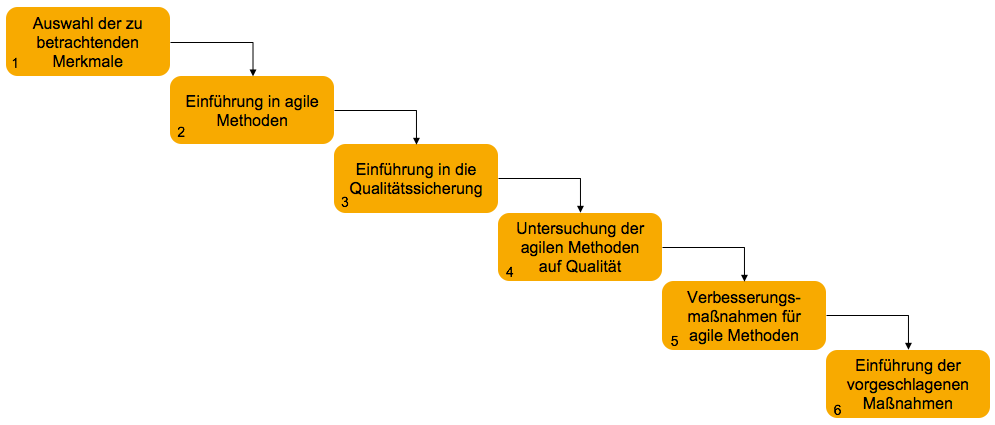
\includegraphics[width=\textwidth]{Abbildungen/ablauf}
                    \caption{Vorgehensweise dieser Arbeit}
                    \label{abb:ablauf}
                \end{center}
        \end{figure}

        Um die Qualität einer Software zu erfassen, müssen Kriterien gegeben sein, anhand derer sie bewertet wird. In Schritt 1 der Abbildung wird zunächst die Qualität definiert und anschließend werden Merkmale definiert, die für qualitative Software betrachtet werden müssen. Aus diesen Merkmalen werden die für die Bausparkasse Relevantesten ausgewählt und im weiteren Rahmen dieser Arbeit betrachtet.

        In \autoref{cha:vorgehensmodelle} werden Softwareprojekte definiert und als Beispiel für eine klassische Herangehensweise das Wasserfallmodell vorgestellt. Im Anschluss wird der Fokus auf agile Verfahren gelegt, wobei zunächst die Prinzipien des agilen Manifests und anschließend verschiedene agile Softwareentwicklungsprozesse erläutert werden. Die agilen Prozesse bilden die Grundlage der Analyse dieser Arbeit und sollen optimiert werden.

        Im folgenden Kapitel wird eine Einführung in die Qualitätssicherung gegeben. Hier wird zwischen verschiedenen qualitätssichernden Maßnahmen differenziert und es werden ausgewählte Methoden zur Sicherstellung und Verbesserung der Qualität im Softwareentstehungsprozess aufgezeigt. Teile dieser Methoden sollen auf die agilen Entwicklungsprozesse angewandt werden, um die Qualität in agilen Prozessen zu verbessern und eine umfassende Sicherung der Qualität zu gewährleisten.

        In \autoref{cha:prozessentwicklung} (Schritt 4) werden die agilen Entwicklungsverfahren beleuchtet und Stärken und Schwächen aufgedeckt. Auf Basis der qualitätssichernden Maßnahmen aus \autoref{cha:einfuehrungQS} werden die agilen Entwicklungsverfahren in Schritt 5 ergänzt. Dies dient als Orientierungshilfe zur qualitätssichernden Erweiterung von agilen Prozessen.

        Damit dieser Prozess kontrolliert und ordnungsgemäß durchgeführt wird, werden erneut Qualitätssicherungsmodelle aus \autoref{sec:qsmethoden} angewandt. Der Soll-Prozess wird mit jeder Iteration kontrolliert und verbessert, damit das Ergebnis des Projekts möglichst alle Anforderungen erfüllt. Die Vorgehensweise hierfür wird skizziert.

        Zum Abschluss werden die Arbeitsergebnisse kritisch bewertet und Möglichkeiten aufgezeigt, diese in der Praxis anzuwenden. 